\section{Introduction: Making Search Feel More Natural}
Despite the ubiquity of online search, help-seeking remains a tedious and difficult process for many, because people are often reluctant to take their hands off the current task to search for help when they need it. Although RePlay's contextual search helped people spend less time once they decided to search, there was still an initial barrier that discouraged many from searching. Creating good search queries can be prohibitively difficult for novices, who may not know the domain vocabulary \cite{Russell2011}. It also switches the user's attention from the task at hand to the task of articulating their goal in a way that will match the resources they seek \cite{Tuovinen1999}. How might we lower the barrier to searching and make it easier for people to find the resources they need in the moment?

When people help each other, they use language, gestures, and shared context to communicate. In contrast, interacting with search engines to find help is still primarily text-based. This chapter explores how multimodal interaction might make searching easier, by enabling people to articulate their thoughts like they would with each other. Different types of information lend themselves better to different modalities; leveraging the strengths of multiple modalities and integrating them smoothly can be extremely effective \cite{Oviatt1999}. 

\begin{figure}[b!]
\centering
  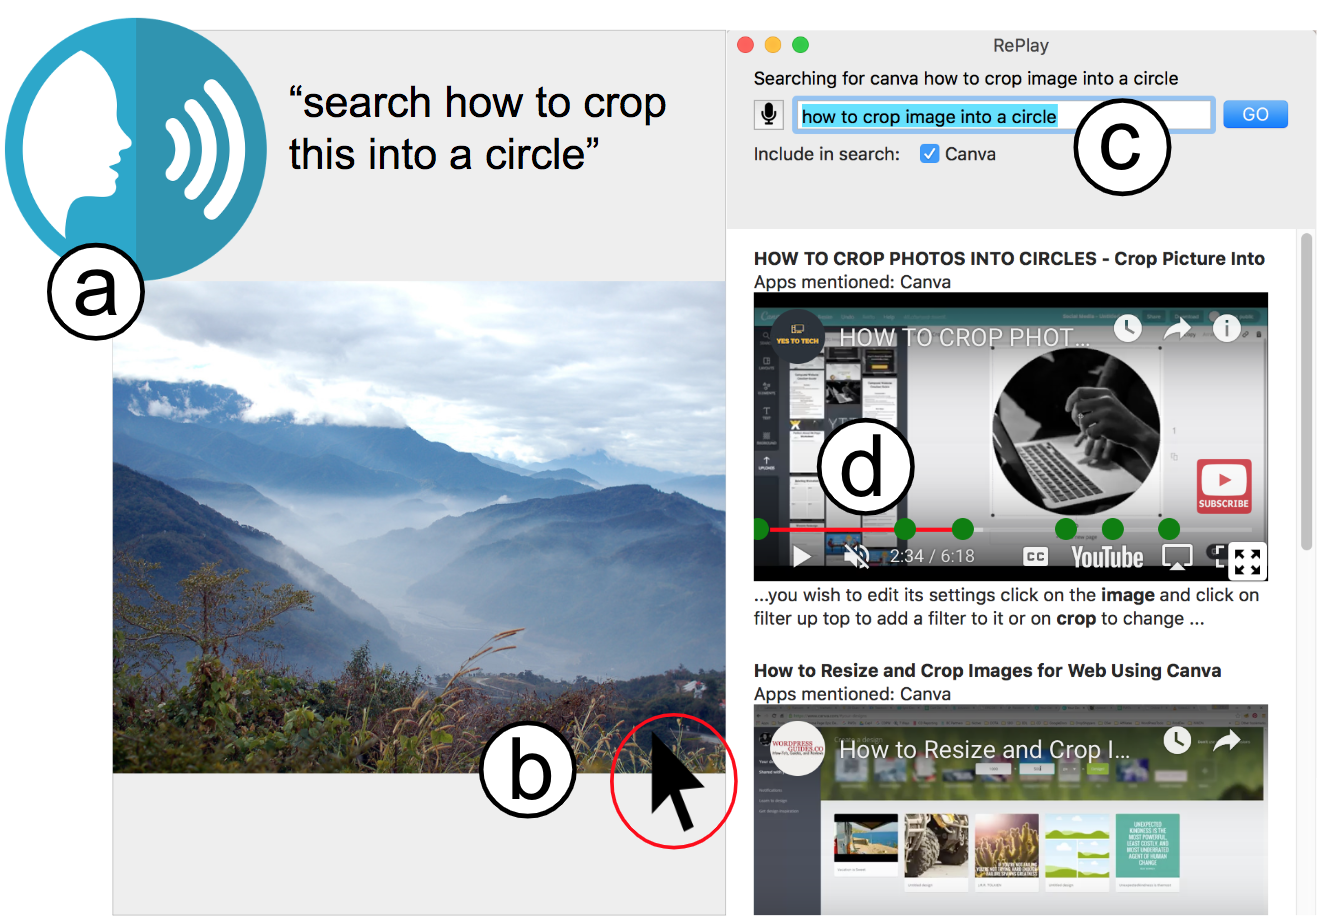
\includegraphics[width=.7\textwidth]{remap/figures/interface.png}
  \caption[ReMap is a multimodal search interface for finding learning videos.]{ReMap is a multimodal search interface for finding learning videos. a) The user speaks their query. b) The user clicks on an image on the canvas while saying the word ``this.'' c) ReMap automatically changes the word ``this'' to ``image.'' d) ReMap highlights relevant moments by placing markers on the timeline of each video result.}~\label{fig:remap_interface}
\end{figure}

We introduce ReMap, a multimodal interface for users to search for learning videos using speech and pointing, without taking their hands (or mouse) off their current task. ReMap builds on RePlay (Chapter \ref{chapter:replay}), which uses relevant context from the user's activities to improve the relevance of search results. ReMap's multimodal help search demonstrates three main design insights:
\begin{enumerate}
\item To avoid context-switching, users can initiate and dictate a search using speech.
\item To avoid needing to learn or recall app-specific terminology, users can point at relevant software elements to include their names in the search query.
\item To simultaneously work on their task while following along with a tutorial, users can play, pause, and navigate video results using speech.
\end{enumerate}

A study with 13 participants found that ReMap allows people to stay focused on their task while help-seeking. The study, along with iterative prototyping and pilot testing, also raised a number of important challenges with incorporating multimodal features into a help-seeking system. We conclude this chapter by discussing ways future work can integrate multimodal search even more smoothly into creative tasks, further lowering the barrier to help-seeking.